% ================================================================
% The printable version of latex/starters/targeted/KS3/statistics/introducingAveragesStarters.tex
%
% This is the same deck, laid out to be handed out rather than put on
% the board. Every slide is shown as it stands before any answer is
% revealed, and 4 copies of it go on one page of A4, two by two, so
% that a printed page cuts into four question sheets.
%
%   made from           latex/starters/targeted/KS3/statistics/introducingAveragesStarters.tex
%   slides on the sheet 5
%   copies of each      4, two by two on A4 landscape
%   printing rules      version 1
%
% Nothing was reworded and nothing was rewritten. Each slide is the slide
% from the deck, asked for at its first step, which is how the answers
% stay hidden.
%
% Please don't edit this file. It is written again from the one it was
% made from whenever that changes, so an edit here would be lost - edit
% that file instead and this one follows.
% ================================================================
\documentclass{beamer}
\usepackage{tikz}
\usetikzlibrary{calc,arrows.meta,patterns}
\usepackage{xcolor}
\usepackage{multicol}
\usepackage{amsmath}

% ================================================================
% Answer-overlay helpers
% ================================================================
\newcommand{\ablank}[1]{%
  \alt<2>{\textcolor{red}{#1}}{\underline{\phantom{#1}}}%
}
\newcommand{\ashow}[1]{\uncover<2->{\textcolor{red}{\small #1}}}
\newcommand{\ashowq}[1]{\alt<2->{\textcolor{red}{\small #1}}{?}}

% Answers drawn straight on to a TikZ diagram, revealed on overlay 2 like \ashow.
% Space is reserved on overlay 1, so the diagram does not move between slides.
\usetikzlibrary{overlay-beamer-styles}
\tikzset{
  ans/.style     = {red, thick, visible on=<2->},
  ansfill/.style = {red!15, visible on=<2->},
  anslab/.style  = {red, font=\tiny, visible on=<2->},
}

\title{Averages: Mean \& Median}
\author{}
\date{}

% Lego tower: \legotower{x-offset}{height}{colour}
% Each brick is 0.65 wide x 0.55 tall, with two studs
\newcommand{\legotower}[3]{%
  \foreach \i in {1,...,#2}{%
    \draw[fill=#3!55, draw=#3!80!black, line width=0.35pt]
      (#1, {(\i-1)*0.55}) rectangle (#1+0.65, {\i*0.55});
    \draw[fill=#3!80, draw=#3!80!black, line width=0.2pt]
      (#1+0.15,{(\i-1)*0.55+0.38}) circle (0.08);
    \draw[fill=#3!80, draw=#3!80!black, line width=0.2pt]
      (#1+0.44,{(\i-1)*0.55+0.38}) circle (0.08);
  }%
}

  \newcommand{\lego}[3]{%
    \foreach \ii in {1,...,#2}{%
      \draw[fill=#3!55,draw=#3!80!black,line width=0.3pt]
        (#1,{(\ii-1)*0.42}) rectangle (#1+0.6,{\ii*0.42});
      \draw[fill=#3!80,draw=#3!80!black,line width=0.15pt]
        (#1+0.13,{(\ii-1)*0.42+0.30}) circle (0.07);
      \draw[fill=#3!80,draw=#3!80!black,line width=0.15pt]
        (#1+0.40,{(\ii-1)*0.42+0.30}) circle (0.07);
    }%
  }


  \newcommand{\legob}[3]{%
    \foreach \ii in {1,...,#2}{%
      \draw[fill=#3!55,draw=#3!80!black,line width=0.3pt]
        (#1,{(\ii-1)*0.42}) rectangle (#1+0.6,{\ii*0.42});
      \draw[fill=#3!80,draw=#3!80!black,line width=0.15pt]
        (#1+0.13,{(\ii-1)*0.42+0.30}) circle (0.07);
      \draw[fill=#3!80,draw=#3!80!black,line width=0.15pt]
        (#1+0.40,{(\ii-1)*0.42+0.30}) circle (0.07);
    }%
  }

% ---------------------------------------------------------------
% Added so this deck prints four slides to a page. Nothing above
% this line was changed.
% ---------------------------------------------------------------
\usepackage{pgfpages}

% 4 slides to a sheet of A4, two by two, with a thin line round each
% so that the page can be cut up. The margin is wide enough that the lines
% fall inside what a printer can actually put ink on.
\pgfpagesuselayout{4 on 1}[a4paper,landscape,border shrink=10mm]
\pgfpageslogicalpageoptions{1}{border code=\pgfusepath{stroke}}
\pgfpageslogicalpageoptions{2}{border code=\pgfusepath{stroke}}
\pgfpageslogicalpageoptions{3}{border code=\pgfusepath{stroke}}
\pgfpageslogicalpageoptions{4}{border code=\pgfusepath{stroke}}

% There is nothing on paper to click, and a slide announcing a new section
% would sit between two copies of the same question and put every page after
% it out of step with the grid.
\setbeamertemplate{navigation symbols}{}
\AtBeginPart{}
\AtBeginSection{}
\AtBeginSubsection{}
\AtBeginSubsubsection{}
\begin{document}

\frame{\titlepage}

%------------------------------------------------
% STARTER 1
%------------------------------------------------
\begin{frame}<1>{Starter}
\vspace{-0.8em}
\begin{columns}[T]

\column{0.33\textwidth}
\begin{center}

% Diagram 1: towers 1,3,2  (scale 0.9, bricks 0.5 tall)
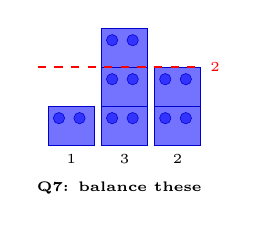
\begin{tikzpicture}[scale=0.9]
  \legotower{0.00}{1}{blue}
  \legotower{0.75}{3}{blue}
  \legotower{1.50}{2}{blue}
  \node[below,font=\tiny] at (0.325,0) {1};
  \node[below,font=\tiny] at (1.075,0) {3};
  \node[below,font=\tiny] at (1.825,0) {2};
  \node[below,font=\tiny\bfseries] at (1.0,{-0.38})
    {\textbf{Q7}: balance these};
  \draw[ans, dashed] (-0.15,1.1) -- (2.15,1.1);
  \node[anslab, right] at (2.15,1.1) {2};
\end{tikzpicture}

\vspace{0.55em}

% Diagram 2: towers 1,3,5,3,3  (scale 0.78 to fit width)
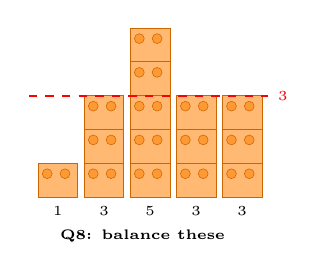
\begin{tikzpicture}[scale=0.78]
  \legotower{0.00}{1}{orange}
  \legotower{0.75}{3}{orange}
  \legotower{1.50}{5}{orange}
  \legotower{2.25}{3}{orange}
  \legotower{3.00}{3}{orange}
  \node[below,font=\tiny] at (0.325,0) {1};
  \node[below,font=\tiny] at (1.075,0) {3};
  \node[below,font=\tiny] at (1.825,0) {5};
  \node[below,font=\tiny] at (2.575,0) {3};
  \node[below,font=\tiny] at (3.325,0) {3};
  \node[below,font=\tiny\bfseries] at (1.7,{-0.38})
    {\textbf{Q8}: balance these};
  \draw[ans, dashed] (-0.15,1.65) -- (3.75,1.65);
  \node[anslab, right] at (3.75,1.65) {3};
\end{tikzpicture}

\end{center}

\column{0.67\textwidth}
\footnotesize
\vspace{0.2em}
\begin{enumerate}\itemsep1pt
  \begin{multicols}{2}
    \item $12 \div 4 = \ashowq{3}$
    \item $18 \div 3 = \ashowq{6}$
  \end{multicols}
  \begin{multicols}{2}
    \item $15 \div 3 = \ashowq{5}$
    \item $28 \div 4 = \ashowq{7}$
  \end{multicols}
  \item Four friends share 20 sweets equally. How many do they each get? \ashow{5 sweets}
  \item Three children have 2, 5 and 8 stickers. They combine them and share them equally. How many does each child get? \ashow{5 stickers}
  \item Draw a picture of the top towers (left), balanced to the same height without changing the total number of bricks.
  \item Draw a picture of the bottom towers (left), balanced to the same height without changing the total number of bricks.
\end{enumerate}

\end{columns}
\end{frame}
\begin{frame}<1>{Starter}
\vspace{-0.8em}
\begin{columns}[T]

\column{0.33\textwidth}
\begin{center}

% Diagram 1: towers 1,3,2  (scale 0.9, bricks 0.5 tall)
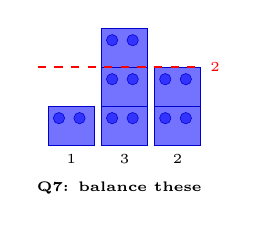
\begin{tikzpicture}[scale=0.9]
  \legotower{0.00}{1}{blue}
  \legotower{0.75}{3}{blue}
  \legotower{1.50}{2}{blue}
  \node[below,font=\tiny] at (0.325,0) {1};
  \node[below,font=\tiny] at (1.075,0) {3};
  \node[below,font=\tiny] at (1.825,0) {2};
  \node[below,font=\tiny\bfseries] at (1.0,{-0.38})
    {\textbf{Q7}: balance these};
  \draw[ans, dashed] (-0.15,1.1) -- (2.15,1.1);
  \node[anslab, right] at (2.15,1.1) {2};
\end{tikzpicture}

\vspace{0.55em}

% Diagram 2: towers 1,3,5,3,3  (scale 0.78 to fit width)
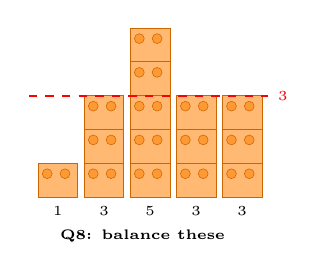
\begin{tikzpicture}[scale=0.78]
  \legotower{0.00}{1}{orange}
  \legotower{0.75}{3}{orange}
  \legotower{1.50}{5}{orange}
  \legotower{2.25}{3}{orange}
  \legotower{3.00}{3}{orange}
  \node[below,font=\tiny] at (0.325,0) {1};
  \node[below,font=\tiny] at (1.075,0) {3};
  \node[below,font=\tiny] at (1.825,0) {5};
  \node[below,font=\tiny] at (2.575,0) {3};
  \node[below,font=\tiny] at (3.325,0) {3};
  \node[below,font=\tiny\bfseries] at (1.7,{-0.38})
    {\textbf{Q8}: balance these};
  \draw[ans, dashed] (-0.15,1.65) -- (3.75,1.65);
  \node[anslab, right] at (3.75,1.65) {3};
\end{tikzpicture}

\end{center}

\column{0.67\textwidth}
\footnotesize
\vspace{0.2em}
\begin{enumerate}\itemsep1pt
  \begin{multicols}{2}
    \item $12 \div 4 = \ashowq{3}$
    \item $18 \div 3 = \ashowq{6}$
  \end{multicols}
  \begin{multicols}{2}
    \item $15 \div 3 = \ashowq{5}$
    \item $28 \div 4 = \ashowq{7}$
  \end{multicols}
  \item Four friends share 20 sweets equally. How many do they each get? \ashow{5 sweets}
  \item Three children have 2, 5 and 8 stickers. They combine them and share them equally. How many does each child get? \ashow{5 stickers}
  \item Draw a picture of the top towers (left), balanced to the same height without changing the total number of bricks.
  \item Draw a picture of the bottom towers (left), balanced to the same height without changing the total number of bricks.
\end{enumerate}

\end{columns}
\end{frame}
\begin{frame}<1>{Starter}
\vspace{-0.8em}
\begin{columns}[T]

\column{0.33\textwidth}
\begin{center}

% Diagram 1: towers 1,3,2  (scale 0.9, bricks 0.5 tall)
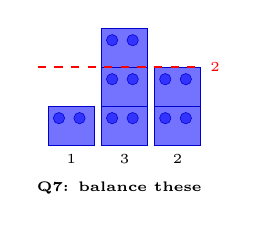
\begin{tikzpicture}[scale=0.9]
  \legotower{0.00}{1}{blue}
  \legotower{0.75}{3}{blue}
  \legotower{1.50}{2}{blue}
  \node[below,font=\tiny] at (0.325,0) {1};
  \node[below,font=\tiny] at (1.075,0) {3};
  \node[below,font=\tiny] at (1.825,0) {2};
  \node[below,font=\tiny\bfseries] at (1.0,{-0.38})
    {\textbf{Q7}: balance these};
  \draw[ans, dashed] (-0.15,1.1) -- (2.15,1.1);
  \node[anslab, right] at (2.15,1.1) {2};
\end{tikzpicture}

\vspace{0.55em}

% Diagram 2: towers 1,3,5,3,3  (scale 0.78 to fit width)
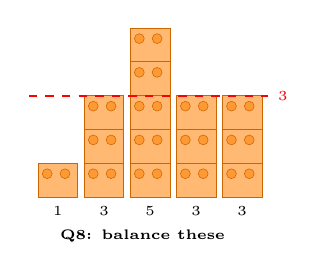
\begin{tikzpicture}[scale=0.78]
  \legotower{0.00}{1}{orange}
  \legotower{0.75}{3}{orange}
  \legotower{1.50}{5}{orange}
  \legotower{2.25}{3}{orange}
  \legotower{3.00}{3}{orange}
  \node[below,font=\tiny] at (0.325,0) {1};
  \node[below,font=\tiny] at (1.075,0) {3};
  \node[below,font=\tiny] at (1.825,0) {5};
  \node[below,font=\tiny] at (2.575,0) {3};
  \node[below,font=\tiny] at (3.325,0) {3};
  \node[below,font=\tiny\bfseries] at (1.7,{-0.38})
    {\textbf{Q8}: balance these};
  \draw[ans, dashed] (-0.15,1.65) -- (3.75,1.65);
  \node[anslab, right] at (3.75,1.65) {3};
\end{tikzpicture}

\end{center}

\column{0.67\textwidth}
\footnotesize
\vspace{0.2em}
\begin{enumerate}\itemsep1pt
  \begin{multicols}{2}
    \item $12 \div 4 = \ashowq{3}$
    \item $18 \div 3 = \ashowq{6}$
  \end{multicols}
  \begin{multicols}{2}
    \item $15 \div 3 = \ashowq{5}$
    \item $28 \div 4 = \ashowq{7}$
  \end{multicols}
  \item Four friends share 20 sweets equally. How many do they each get? \ashow{5 sweets}
  \item Three children have 2, 5 and 8 stickers. They combine them and share them equally. How many does each child get? \ashow{5 stickers}
  \item Draw a picture of the top towers (left), balanced to the same height without changing the total number of bricks.
  \item Draw a picture of the bottom towers (left), balanced to the same height without changing the total number of bricks.
\end{enumerate}

\end{columns}
\end{frame}
\begin{frame}<1>{Starter}
\vspace{-0.8em}
\begin{columns}[T]

\column{0.33\textwidth}
\begin{center}

% Diagram 1: towers 1,3,2  (scale 0.9, bricks 0.5 tall)
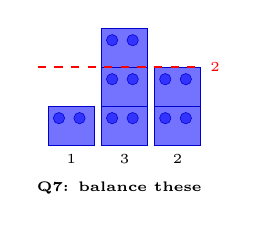
\begin{tikzpicture}[scale=0.9]
  \legotower{0.00}{1}{blue}
  \legotower{0.75}{3}{blue}
  \legotower{1.50}{2}{blue}
  \node[below,font=\tiny] at (0.325,0) {1};
  \node[below,font=\tiny] at (1.075,0) {3};
  \node[below,font=\tiny] at (1.825,0) {2};
  \node[below,font=\tiny\bfseries] at (1.0,{-0.38})
    {\textbf{Q7}: balance these};
  \draw[ans, dashed] (-0.15,1.1) -- (2.15,1.1);
  \node[anslab, right] at (2.15,1.1) {2};
\end{tikzpicture}

\vspace{0.55em}

% Diagram 2: towers 1,3,5,3,3  (scale 0.78 to fit width)
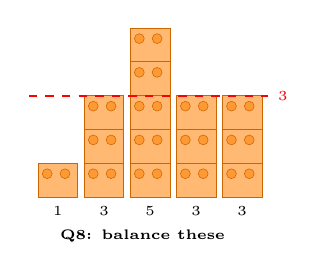
\begin{tikzpicture}[scale=0.78]
  \legotower{0.00}{1}{orange}
  \legotower{0.75}{3}{orange}
  \legotower{1.50}{5}{orange}
  \legotower{2.25}{3}{orange}
  \legotower{3.00}{3}{orange}
  \node[below,font=\tiny] at (0.325,0) {1};
  \node[below,font=\tiny] at (1.075,0) {3};
  \node[below,font=\tiny] at (1.825,0) {5};
  \node[below,font=\tiny] at (2.575,0) {3};
  \node[below,font=\tiny] at (3.325,0) {3};
  \node[below,font=\tiny\bfseries] at (1.7,{-0.38})
    {\textbf{Q8}: balance these};
  \draw[ans, dashed] (-0.15,1.65) -- (3.75,1.65);
  \node[anslab, right] at (3.75,1.65) {3};
\end{tikzpicture}

\end{center}

\column{0.67\textwidth}
\footnotesize
\vspace{0.2em}
\begin{enumerate}\itemsep1pt
  \begin{multicols}{2}
    \item $12 \div 4 = \ashowq{3}$
    \item $18 \div 3 = \ashowq{6}$
  \end{multicols}
  \begin{multicols}{2}
    \item $15 \div 3 = \ashowq{5}$
    \item $28 \div 4 = \ashowq{7}$
  \end{multicols}
  \item Four friends share 20 sweets equally. How many do they each get? \ashow{5 sweets}
  \item Three children have 2, 5 and 8 stickers. They combine them and share them equally. How many does each child get? \ashow{5 stickers}
  \item Draw a picture of the top towers (left), balanced to the same height without changing the total number of bricks.
  \item Draw a picture of the bottom towers (left), balanced to the same height without changing the total number of bricks.
\end{enumerate}

\end{columns}
\end{frame}

%------------------------------------------------
% STARTER 2
%------------------------------------------------
\begin{frame}<1>{Starter}
\vspace{-0.8em}
\begin{columns}[T]

\column{0.33\textwidth}
\begin{center}

% Diagram 1: towers 3,5,4,8 — brick height 0.42 to keep 8-tower in frame
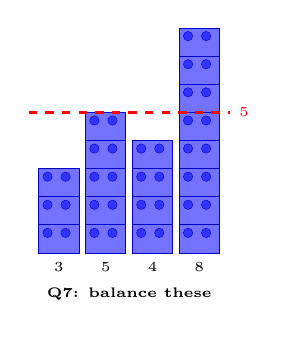
\begin{tikzpicture}[scale=0.85]

  \lego{0.00}{3}{blue}
  \lego{0.70}{5}{blue}
  \lego{1.40}{4}{blue}
  \lego{2.10}{8}{blue}
  \node[below,font=\tiny] at (0.30,0) {3};
  \node[below,font=\tiny] at (1.00,0) {5};
  \node[below,font=\tiny] at (1.70,0) {4};
  \node[below,font=\tiny] at (2.40,0) {8};
  \node[below,font=\tiny\bfseries] at (1.35,{-0.38})
    {\textbf{Q7}: balance these};
  \draw[ans, dashed] (-0.15,2.10) -- (2.85,2.10);
  \node[anslab, right] at (2.85,2.10) {5};
\end{tikzpicture}

\vspace{0.45em}

% Diagram 2: towers 1,5,2,8,4
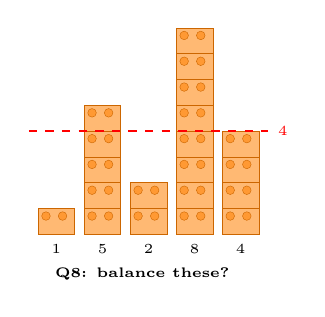
\begin{tikzpicture}[scale=0.78]

  \legob{0.00}{1}{orange}
  \legob{0.75}{5}{orange}
  \legob{1.50}{2}{orange}
  \legob{2.25}{8}{orange}
  \legob{3.00}{4}{orange}
  \node[below,font=\tiny] at (0.30,0) {1};
  \node[below,font=\tiny] at (1.05,0) {5};
  \node[below,font=\tiny] at (1.80,0) {2};
  \node[below,font=\tiny] at (2.55,0) {8};
  \node[below,font=\tiny] at (3.30,0) {4};
  \node[below,font=\tiny\bfseries] at (1.7,{-0.38})
    {\textbf{Q8}: balance these?};
  \draw[ans, dashed] (-0.15,1.68) -- (3.75,1.68);
  \node[anslab, right] at (3.75,1.68) {4};
\end{tikzpicture}

\end{center}

\column{0.67\textwidth}
\footnotesize
\vspace{0.2em}
  \begin{multicols}{2}
  \begin{enumerate}
    \item $7 \times 8 = \ashowq{56}$
    \item $63 \div 7 = \ashowq{9}$
    \end{enumerate}
  \end{multicols}
  \begin{multicols}{2}
  \begin{enumerate}
  \setcounter{enumi}{2}
    \item $48 \div 8 = \ashowq{6}$
    \item $5 \times 9 = \ashowq{45}$
    \end{enumerate}
  \end{multicols}
  \begin{enumerate}
  \setcounter{enumi}{4}
  \item Five children have 4, 7, 3, 6, 5 marbles. Shared equally, how many each? \ashow{5 marbles}
  \item Six friends earn £8, £14, £10, £6, £12, £10 at a car wash. Split fairly — how much each? \ashow{\pounds10 each}
  \item Eight runners finish in 54, 48, 61, 57, 50, 63, 55, 52 s. Without doing any calculations, estimate the average time. \ashow{about 55 s}
  \item What heights would the top towers balance out to? \ashow{5 bricks high}
  \item What heights would the bottom towers balance out to? \ashow{4 bricks high}
\end{enumerate}

\end{columns}
\end{frame}
\begin{frame}<1>{Starter}
\vspace{-0.8em}
\begin{columns}[T]

\column{0.33\textwidth}
\begin{center}

% Diagram 1: towers 3,5,4,8 — brick height 0.42 to keep 8-tower in frame
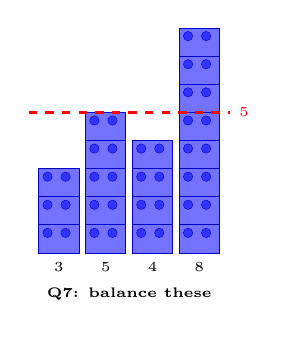
\begin{tikzpicture}[scale=0.85]

  \lego{0.00}{3}{blue}
  \lego{0.70}{5}{blue}
  \lego{1.40}{4}{blue}
  \lego{2.10}{8}{blue}
  \node[below,font=\tiny] at (0.30,0) {3};
  \node[below,font=\tiny] at (1.00,0) {5};
  \node[below,font=\tiny] at (1.70,0) {4};
  \node[below,font=\tiny] at (2.40,0) {8};
  \node[below,font=\tiny\bfseries] at (1.35,{-0.38})
    {\textbf{Q7}: balance these};
  \draw[ans, dashed] (-0.15,2.10) -- (2.85,2.10);
  \node[anslab, right] at (2.85,2.10) {5};
\end{tikzpicture}

\vspace{0.45em}

% Diagram 2: towers 1,5,2,8,4
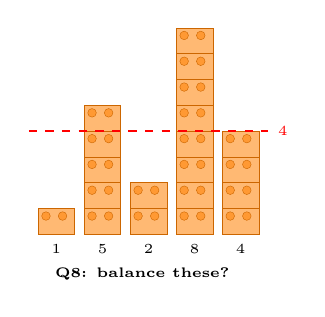
\begin{tikzpicture}[scale=0.78]

  \legob{0.00}{1}{orange}
  \legob{0.75}{5}{orange}
  \legob{1.50}{2}{orange}
  \legob{2.25}{8}{orange}
  \legob{3.00}{4}{orange}
  \node[below,font=\tiny] at (0.30,0) {1};
  \node[below,font=\tiny] at (1.05,0) {5};
  \node[below,font=\tiny] at (1.80,0) {2};
  \node[below,font=\tiny] at (2.55,0) {8};
  \node[below,font=\tiny] at (3.30,0) {4};
  \node[below,font=\tiny\bfseries] at (1.7,{-0.38})
    {\textbf{Q8}: balance these?};
  \draw[ans, dashed] (-0.15,1.68) -- (3.75,1.68);
  \node[anslab, right] at (3.75,1.68) {4};
\end{tikzpicture}

\end{center}

\column{0.67\textwidth}
\footnotesize
\vspace{0.2em}
  \begin{multicols}{2}
  \begin{enumerate}
    \item $7 \times 8 = \ashowq{56}$
    \item $63 \div 7 = \ashowq{9}$
    \end{enumerate}
  \end{multicols}
  \begin{multicols}{2}
  \begin{enumerate}
  \setcounter{enumi}{2}
    \item $48 \div 8 = \ashowq{6}$
    \item $5 \times 9 = \ashowq{45}$
    \end{enumerate}
  \end{multicols}
  \begin{enumerate}
  \setcounter{enumi}{4}
  \item Five children have 4, 7, 3, 6, 5 marbles. Shared equally, how many each? \ashow{5 marbles}
  \item Six friends earn £8, £14, £10, £6, £12, £10 at a car wash. Split fairly — how much each? \ashow{\pounds10 each}
  \item Eight runners finish in 54, 48, 61, 57, 50, 63, 55, 52 s. Without doing any calculations, estimate the average time. \ashow{about 55 s}
  \item What heights would the top towers balance out to? \ashow{5 bricks high}
  \item What heights would the bottom towers balance out to? \ashow{4 bricks high}
\end{enumerate}

\end{columns}
\end{frame}
\begin{frame}<1>{Starter}
\vspace{-0.8em}
\begin{columns}[T]

\column{0.33\textwidth}
\begin{center}

% Diagram 1: towers 3,5,4,8 — brick height 0.42 to keep 8-tower in frame
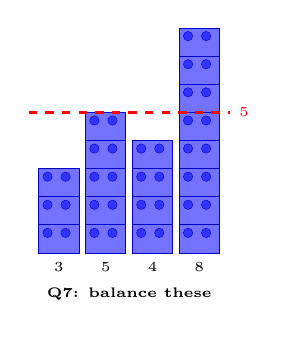
\begin{tikzpicture}[scale=0.85]

  \lego{0.00}{3}{blue}
  \lego{0.70}{5}{blue}
  \lego{1.40}{4}{blue}
  \lego{2.10}{8}{blue}
  \node[below,font=\tiny] at (0.30,0) {3};
  \node[below,font=\tiny] at (1.00,0) {5};
  \node[below,font=\tiny] at (1.70,0) {4};
  \node[below,font=\tiny] at (2.40,0) {8};
  \node[below,font=\tiny\bfseries] at (1.35,{-0.38})
    {\textbf{Q7}: balance these};
  \draw[ans, dashed] (-0.15,2.10) -- (2.85,2.10);
  \node[anslab, right] at (2.85,2.10) {5};
\end{tikzpicture}

\vspace{0.45em}

% Diagram 2: towers 1,5,2,8,4
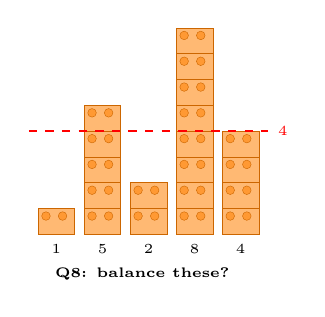
\begin{tikzpicture}[scale=0.78]

  \legob{0.00}{1}{orange}
  \legob{0.75}{5}{orange}
  \legob{1.50}{2}{orange}
  \legob{2.25}{8}{orange}
  \legob{3.00}{4}{orange}
  \node[below,font=\tiny] at (0.30,0) {1};
  \node[below,font=\tiny] at (1.05,0) {5};
  \node[below,font=\tiny] at (1.80,0) {2};
  \node[below,font=\tiny] at (2.55,0) {8};
  \node[below,font=\tiny] at (3.30,0) {4};
  \node[below,font=\tiny\bfseries] at (1.7,{-0.38})
    {\textbf{Q8}: balance these?};
  \draw[ans, dashed] (-0.15,1.68) -- (3.75,1.68);
  \node[anslab, right] at (3.75,1.68) {4};
\end{tikzpicture}

\end{center}

\column{0.67\textwidth}
\footnotesize
\vspace{0.2em}
  \begin{multicols}{2}
  \begin{enumerate}
    \item $7 \times 8 = \ashowq{56}$
    \item $63 \div 7 = \ashowq{9}$
    \end{enumerate}
  \end{multicols}
  \begin{multicols}{2}
  \begin{enumerate}
  \setcounter{enumi}{2}
    \item $48 \div 8 = \ashowq{6}$
    \item $5 \times 9 = \ashowq{45}$
    \end{enumerate}
  \end{multicols}
  \begin{enumerate}
  \setcounter{enumi}{4}
  \item Five children have 4, 7, 3, 6, 5 marbles. Shared equally, how many each? \ashow{5 marbles}
  \item Six friends earn £8, £14, £10, £6, £12, £10 at a car wash. Split fairly — how much each? \ashow{\pounds10 each}
  \item Eight runners finish in 54, 48, 61, 57, 50, 63, 55, 52 s. Without doing any calculations, estimate the average time. \ashow{about 55 s}
  \item What heights would the top towers balance out to? \ashow{5 bricks high}
  \item What heights would the bottom towers balance out to? \ashow{4 bricks high}
\end{enumerate}

\end{columns}
\end{frame}
\begin{frame}<1>{Starter}
\vspace{-0.8em}
\begin{columns}[T]

\column{0.33\textwidth}
\begin{center}

% Diagram 1: towers 3,5,4,8 — brick height 0.42 to keep 8-tower in frame
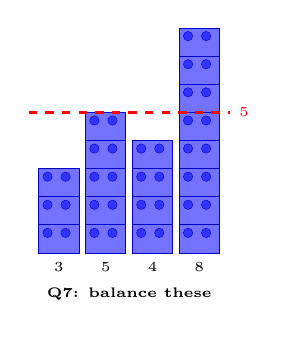
\begin{tikzpicture}[scale=0.85]

  \lego{0.00}{3}{blue}
  \lego{0.70}{5}{blue}
  \lego{1.40}{4}{blue}
  \lego{2.10}{8}{blue}
  \node[below,font=\tiny] at (0.30,0) {3};
  \node[below,font=\tiny] at (1.00,0) {5};
  \node[below,font=\tiny] at (1.70,0) {4};
  \node[below,font=\tiny] at (2.40,0) {8};
  \node[below,font=\tiny\bfseries] at (1.35,{-0.38})
    {\textbf{Q7}: balance these};
  \draw[ans, dashed] (-0.15,2.10) -- (2.85,2.10);
  \node[anslab, right] at (2.85,2.10) {5};
\end{tikzpicture}

\vspace{0.45em}

% Diagram 2: towers 1,5,2,8,4
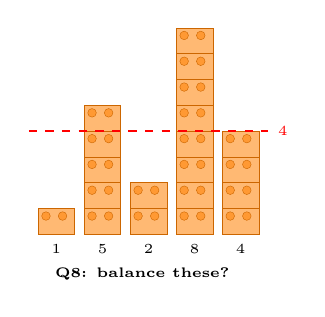
\begin{tikzpicture}[scale=0.78]

  \legob{0.00}{1}{orange}
  \legob{0.75}{5}{orange}
  \legob{1.50}{2}{orange}
  \legob{2.25}{8}{orange}
  \legob{3.00}{4}{orange}
  \node[below,font=\tiny] at (0.30,0) {1};
  \node[below,font=\tiny] at (1.05,0) {5};
  \node[below,font=\tiny] at (1.80,0) {2};
  \node[below,font=\tiny] at (2.55,0) {8};
  \node[below,font=\tiny] at (3.30,0) {4};
  \node[below,font=\tiny\bfseries] at (1.7,{-0.38})
    {\textbf{Q8}: balance these?};
  \draw[ans, dashed] (-0.15,1.68) -- (3.75,1.68);
  \node[anslab, right] at (3.75,1.68) {4};
\end{tikzpicture}

\end{center}

\column{0.67\textwidth}
\footnotesize
\vspace{0.2em}
  \begin{multicols}{2}
  \begin{enumerate}
    \item $7 \times 8 = \ashowq{56}$
    \item $63 \div 7 = \ashowq{9}$
    \end{enumerate}
  \end{multicols}
  \begin{multicols}{2}
  \begin{enumerate}
  \setcounter{enumi}{2}
    \item $48 \div 8 = \ashowq{6}$
    \item $5 \times 9 = \ashowq{45}$
    \end{enumerate}
  \end{multicols}
  \begin{enumerate}
  \setcounter{enumi}{4}
  \item Five children have 4, 7, 3, 6, 5 marbles. Shared equally, how many each? \ashow{5 marbles}
  \item Six friends earn £8, £14, £10, £6, £12, £10 at a car wash. Split fairly — how much each? \ashow{\pounds10 each}
  \item Eight runners finish in 54, 48, 61, 57, 50, 63, 55, 52 s. Without doing any calculations, estimate the average time. \ashow{about 55 s}
  \item What heights would the top towers balance out to? \ashow{5 bricks high}
  \item What heights would the bottom towers balance out to? \ashow{4 bricks high}
\end{enumerate}

\end{columns}
\end{frame}

%------------------------------------------------
% STARTER 3
%------------------------------------------------
\begin{frame}<1>{Starter}
\vspace{-0.8em}

\footnotesize
\vspace{0.2em}
\begin{enumerate}\itemsep1pt
  \begin{multicols}{2}
    \item $3 + 4 + 7 = \ashowq{14}$
    \item $15+27+18=\ashowq{60}$
    \item $60\div 4=\ashowq{15}$
    \item $-15 \div 3=\ashowq{-5}$
  \end{multicols}
  \vspace{-1em}
  \item What is the mean of: $4,\ 6,\ 2,\ 8$ \ashow{5}
  \item What is the mean  of: $3,\ 9,\ 5,\ 7,\ 1$ \ashow{5}
  \item What is the mean  of: $-3,\ 5,\ -1,\ 7,\ 2$ \ashow{2}
  \item What is the mean  of: $-8,\ -2,\ -5,\ -1,\ -4$ \ashow{$-4$}
\end{enumerate}

\begin{enumerate}\itemsep1pt
  \setcounter{enumi}8
  \item The mean of four numbers is 9. Three are 6, 11 and 8. Find the fourth. \ashow{11}
  \item The mean of $3,\ 7,\ x,\ 10$ is $8$. What is $x$? \ashow{12}
\end{enumerate}


\end{frame}
\begin{frame}<1>{Starter}
\vspace{-0.8em}

\footnotesize
\vspace{0.2em}
\begin{enumerate}\itemsep1pt
  \begin{multicols}{2}
    \item $3 + 4 + 7 = \ashowq{14}$
    \item $15+27+18=\ashowq{60}$
    \item $60\div 4=\ashowq{15}$
    \item $-15 \div 3=\ashowq{-5}$
  \end{multicols}
  \vspace{-1em}
  \item What is the mean of: $4,\ 6,\ 2,\ 8$ \ashow{5}
  \item What is the mean  of: $3,\ 9,\ 5,\ 7,\ 1$ \ashow{5}
  \item What is the mean  of: $-3,\ 5,\ -1,\ 7,\ 2$ \ashow{2}
  \item What is the mean  of: $-8,\ -2,\ -5,\ -1,\ -4$ \ashow{$-4$}
\end{enumerate}

\begin{enumerate}\itemsep1pt
  \setcounter{enumi}8
  \item The mean of four numbers is 9. Three are 6, 11 and 8. Find the fourth. \ashow{11}
  \item The mean of $3,\ 7,\ x,\ 10$ is $8$. What is $x$? \ashow{12}
\end{enumerate}


\end{frame}
\begin{frame}<1>{Starter}
\vspace{-0.8em}

\footnotesize
\vspace{0.2em}
\begin{enumerate}\itemsep1pt
  \begin{multicols}{2}
    \item $3 + 4 + 7 = \ashowq{14}$
    \item $15+27+18=\ashowq{60}$
    \item $60\div 4=\ashowq{15}$
    \item $-15 \div 3=\ashowq{-5}$
  \end{multicols}
  \vspace{-1em}
  \item What is the mean of: $4,\ 6,\ 2,\ 8$ \ashow{5}
  \item What is the mean  of: $3,\ 9,\ 5,\ 7,\ 1$ \ashow{5}
  \item What is the mean  of: $-3,\ 5,\ -1,\ 7,\ 2$ \ashow{2}
  \item What is the mean  of: $-8,\ -2,\ -5,\ -1,\ -4$ \ashow{$-4$}
\end{enumerate}

\begin{enumerate}\itemsep1pt
  \setcounter{enumi}8
  \item The mean of four numbers is 9. Three are 6, 11 and 8. Find the fourth. \ashow{11}
  \item The mean of $3,\ 7,\ x,\ 10$ is $8$. What is $x$? \ashow{12}
\end{enumerate}


\end{frame}
\begin{frame}<1>{Starter}
\vspace{-0.8em}

\footnotesize
\vspace{0.2em}
\begin{enumerate}\itemsep1pt
  \begin{multicols}{2}
    \item $3 + 4 + 7 = \ashowq{14}$
    \item $15+27+18=\ashowq{60}$
    \item $60\div 4=\ashowq{15}$
    \item $-15 \div 3=\ashowq{-5}$
  \end{multicols}
  \vspace{-1em}
  \item What is the mean of: $4,\ 6,\ 2,\ 8$ \ashow{5}
  \item What is the mean  of: $3,\ 9,\ 5,\ 7,\ 1$ \ashow{5}
  \item What is the mean  of: $-3,\ 5,\ -1,\ 7,\ 2$ \ashow{2}
  \item What is the mean  of: $-8,\ -2,\ -5,\ -1,\ -4$ \ashow{$-4$}
\end{enumerate}

\begin{enumerate}\itemsep1pt
  \setcounter{enumi}8
  \item The mean of four numbers is 9. Three are 6, 11 and 8. Find the fourth. \ashow{11}
  \item The mean of $3,\ 7,\ x,\ 10$ is $8$. What is $x$? \ashow{12}
\end{enumerate}


\end{frame}

%------------------------------------------------
% STARTER 4
%------------------------------------------------
\begin{frame}<1>{Starter 4}
\vspace{-0.8em}

\begin{columns}[T]

% ---------------- LEFT COLUMN ----------------
\column{0.33\textwidth}

\begin{center}

\vspace{7em}

% Dot plot: house prices with outlier
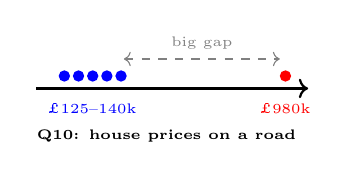
\begin{tikzpicture}[scale=0.72]

  \draw[thick,->] (-0.2,0) -- (4.6,0);

  \foreach \xd in {0.3,0.55,0.8,1.05,1.3}{
    \fill[blue] (\xd,0.22) circle (0.1);
  }

  \fill[red] (4.2,0.22) circle (0.1);

  \node[below,font=\tiny,blue] at (0.8,-0.1)
    {\pounds125--140k};

  \node[below,font=\tiny,red] at (4.2,-0.1)
    {\pounds980k};

  \draw[<->,dashed,gray]
    (1.35,0.52) -- (4.1,0.52)
    node[midway,above,font=\tiny,gray]{big gap};

  \node[below,font=\tiny\bfseries]
    at (2.1,-0.55)
    {\textbf{Q10}: house prices on a road};

\end{tikzpicture}

\end{center}

% ---------------- RIGHT COLUMN ----------------
\column{0.67\textwidth}

\footnotesize
\vspace{0.2em}

% First four quick questions
\begin{multicols}{2}
\begin{enumerate}\itemsep1pt
  \item $4+2+10=\ashowq{16}$
  \item $-4+9=\ashowq{5}$
  \item $-3-5=\ashowq{-8}$
  \item $6\times4=\ashowq{24}$
\end{enumerate}
\end{multicols}

% Remaining questions
\begin{enumerate}\itemsep1pt
\setcounter{enumi}{4}

  \item Order smallest to largest:
  $8,3,11,5,7$.
  Which is the middle value? \ashow{7}

  \item Order:
  $21,14,9,35,17,28,6$.
  Which is the middle value? \ashow{17}

  \item For $3,7,8,9,41$:
  \textit{estimate} whether the middle value is above or below the mean.
  Then check. \ashow{below: median $8$, mean $13.6$}

  \item What is the middle value of:
  $-7,\ -2,\ -5,\ 1,\ -1,\ 3,\ -3$ \ashow{$-2$}

  \item What is the middle value of:
  $\tfrac{1}{2},\ \tfrac{1}{4},\ \tfrac{3}{4},\ \tfrac{1}{8},\ \tfrac{5}{8}$ \ashow{$\frac{1}{2}$}

  \item House prices on a road are:
  \pounds130k,
  \pounds125k,
  \pounds140k,
  \pounds128k,
  \pounds135k,
  \textcolor{red}{\pounds980k}.

  Why might the mean not be helpful? \ashow{the \pounds980k outlier pulls the mean up}

\end{enumerate}

\end{columns}

\end{frame}
\begin{frame}<1>{Starter 4}
\vspace{-0.8em}

\begin{columns}[T]

% ---------------- LEFT COLUMN ----------------
\column{0.33\textwidth}

\begin{center}

\vspace{7em}

% Dot plot: house prices with outlier
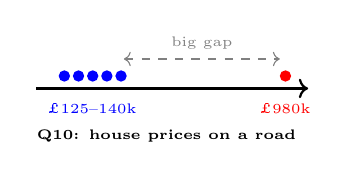
\begin{tikzpicture}[scale=0.72]

  \draw[thick,->] (-0.2,0) -- (4.6,0);

  \foreach \xd in {0.3,0.55,0.8,1.05,1.3}{
    \fill[blue] (\xd,0.22) circle (0.1);
  }

  \fill[red] (4.2,0.22) circle (0.1);

  \node[below,font=\tiny,blue] at (0.8,-0.1)
    {\pounds125--140k};

  \node[below,font=\tiny,red] at (4.2,-0.1)
    {\pounds980k};

  \draw[<->,dashed,gray]
    (1.35,0.52) -- (4.1,0.52)
    node[midway,above,font=\tiny,gray]{big gap};

  \node[below,font=\tiny\bfseries]
    at (2.1,-0.55)
    {\textbf{Q10}: house prices on a road};

\end{tikzpicture}

\end{center}

% ---------------- RIGHT COLUMN ----------------
\column{0.67\textwidth}

\footnotesize
\vspace{0.2em}

% First four quick questions
\begin{multicols}{2}
\begin{enumerate}\itemsep1pt
  \item $4+2+10=\ashowq{16}$
  \item $-4+9=\ashowq{5}$
  \item $-3-5=\ashowq{-8}$
  \item $6\times4=\ashowq{24}$
\end{enumerate}
\end{multicols}

% Remaining questions
\begin{enumerate}\itemsep1pt
\setcounter{enumi}{4}

  \item Order smallest to largest:
  $8,3,11,5,7$.
  Which is the middle value? \ashow{7}

  \item Order:
  $21,14,9,35,17,28,6$.
  Which is the middle value? \ashow{17}

  \item For $3,7,8,9,41$:
  \textit{estimate} whether the middle value is above or below the mean.
  Then check. \ashow{below: median $8$, mean $13.6$}

  \item What is the middle value of:
  $-7,\ -2,\ -5,\ 1,\ -1,\ 3,\ -3$ \ashow{$-2$}

  \item What is the middle value of:
  $\tfrac{1}{2},\ \tfrac{1}{4},\ \tfrac{3}{4},\ \tfrac{1}{8},\ \tfrac{5}{8}$ \ashow{$\frac{1}{2}$}

  \item House prices on a road are:
  \pounds130k,
  \pounds125k,
  \pounds140k,
  \pounds128k,
  \pounds135k,
  \textcolor{red}{\pounds980k}.

  Why might the mean not be helpful? \ashow{the \pounds980k outlier pulls the mean up}

\end{enumerate}

\end{columns}

\end{frame}
\begin{frame}<1>{Starter 4}
\vspace{-0.8em}

\begin{columns}[T]

% ---------------- LEFT COLUMN ----------------
\column{0.33\textwidth}

\begin{center}

\vspace{7em}

% Dot plot: house prices with outlier
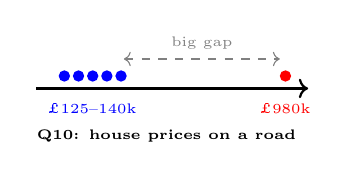
\begin{tikzpicture}[scale=0.72]

  \draw[thick,->] (-0.2,0) -- (4.6,0);

  \foreach \xd in {0.3,0.55,0.8,1.05,1.3}{
    \fill[blue] (\xd,0.22) circle (0.1);
  }

  \fill[red] (4.2,0.22) circle (0.1);

  \node[below,font=\tiny,blue] at (0.8,-0.1)
    {\pounds125--140k};

  \node[below,font=\tiny,red] at (4.2,-0.1)
    {\pounds980k};

  \draw[<->,dashed,gray]
    (1.35,0.52) -- (4.1,0.52)
    node[midway,above,font=\tiny,gray]{big gap};

  \node[below,font=\tiny\bfseries]
    at (2.1,-0.55)
    {\textbf{Q10}: house prices on a road};

\end{tikzpicture}

\end{center}

% ---------------- RIGHT COLUMN ----------------
\column{0.67\textwidth}

\footnotesize
\vspace{0.2em}

% First four quick questions
\begin{multicols}{2}
\begin{enumerate}\itemsep1pt
  \item $4+2+10=\ashowq{16}$
  \item $-4+9=\ashowq{5}$
  \item $-3-5=\ashowq{-8}$
  \item $6\times4=\ashowq{24}$
\end{enumerate}
\end{multicols}

% Remaining questions
\begin{enumerate}\itemsep1pt
\setcounter{enumi}{4}

  \item Order smallest to largest:
  $8,3,11,5,7$.
  Which is the middle value? \ashow{7}

  \item Order:
  $21,14,9,35,17,28,6$.
  Which is the middle value? \ashow{17}

  \item For $3,7,8,9,41$:
  \textit{estimate} whether the middle value is above or below the mean.
  Then check. \ashow{below: median $8$, mean $13.6$}

  \item What is the middle value of:
  $-7,\ -2,\ -5,\ 1,\ -1,\ 3,\ -3$ \ashow{$-2$}

  \item What is the middle value of:
  $\tfrac{1}{2},\ \tfrac{1}{4},\ \tfrac{3}{4},\ \tfrac{1}{8},\ \tfrac{5}{8}$ \ashow{$\frac{1}{2}$}

  \item House prices on a road are:
  \pounds130k,
  \pounds125k,
  \pounds140k,
  \pounds128k,
  \pounds135k,
  \textcolor{red}{\pounds980k}.

  Why might the mean not be helpful? \ashow{the \pounds980k outlier pulls the mean up}

\end{enumerate}

\end{columns}

\end{frame}
\begin{frame}<1>{Starter 4}
\vspace{-0.8em}

\begin{columns}[T]

% ---------------- LEFT COLUMN ----------------
\column{0.33\textwidth}

\begin{center}

\vspace{7em}

% Dot plot: house prices with outlier
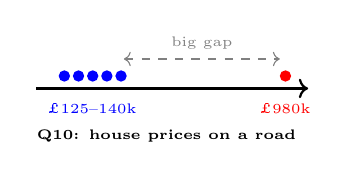
\begin{tikzpicture}[scale=0.72]

  \draw[thick,->] (-0.2,0) -- (4.6,0);

  \foreach \xd in {0.3,0.55,0.8,1.05,1.3}{
    \fill[blue] (\xd,0.22) circle (0.1);
  }

  \fill[red] (4.2,0.22) circle (0.1);

  \node[below,font=\tiny,blue] at (0.8,-0.1)
    {\pounds125--140k};

  \node[below,font=\tiny,red] at (4.2,-0.1)
    {\pounds980k};

  \draw[<->,dashed,gray]
    (1.35,0.52) -- (4.1,0.52)
    node[midway,above,font=\tiny,gray]{big gap};

  \node[below,font=\tiny\bfseries]
    at (2.1,-0.55)
    {\textbf{Q10}: house prices on a road};

\end{tikzpicture}

\end{center}

% ---------------- RIGHT COLUMN ----------------
\column{0.67\textwidth}

\footnotesize
\vspace{0.2em}

% First four quick questions
\begin{multicols}{2}
\begin{enumerate}\itemsep1pt
  \item $4+2+10=\ashowq{16}$
  \item $-4+9=\ashowq{5}$
  \item $-3-5=\ashowq{-8}$
  \item $6\times4=\ashowq{24}$
\end{enumerate}
\end{multicols}

% Remaining questions
\begin{enumerate}\itemsep1pt
\setcounter{enumi}{4}

  \item Order smallest to largest:
  $8,3,11,5,7$.
  Which is the middle value? \ashow{7}

  \item Order:
  $21,14,9,35,17,28,6$.
  Which is the middle value? \ashow{17}

  \item For $3,7,8,9,41$:
  \textit{estimate} whether the middle value is above or below the mean.
  Then check. \ashow{below: median $8$, mean $13.6$}

  \item What is the middle value of:
  $-7,\ -2,\ -5,\ 1,\ -1,\ 3,\ -3$ \ashow{$-2$}

  \item What is the middle value of:
  $\tfrac{1}{2},\ \tfrac{1}{4},\ \tfrac{3}{4},\ \tfrac{1}{8},\ \tfrac{5}{8}$ \ashow{$\frac{1}{2}$}

  \item House prices on a road are:
  \pounds130k,
  \pounds125k,
  \pounds140k,
  \pounds128k,
  \pounds135k,
  \textcolor{red}{\pounds980k}.

  Why might the mean not be helpful? \ashow{the \pounds980k outlier pulls the mean up}

\end{enumerate}

\end{columns}

\end{frame}

%------------------------------------------------
% STARTER 5
%------------------------------------------------
\begin{frame}<1>{Starter}
\vspace{-0.8em}
\begin{columns}[T]

\column{0.33\textwidth}
\begin{center}

\vspace{7em}

% Dot plot showing mean pulled by outlier vs stable median
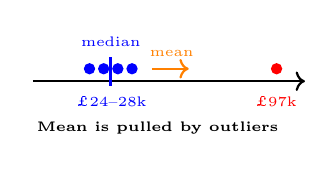
\begin{tikzpicture}[scale=0.72]
  \draw[thick,->] (-0.2,0) -- (4.6,0);
  \foreach \xd in {0.8, 1.05, 1.3, 1.55}{
    \fill[blue] (\xd,0.22) circle (0.1);
  }
  \fill[red] (4.1,0.22) circle (0.1);
  \node[below,font=\tiny,blue] at (1.2,{-0.1})  {£24--28k};
  \node[below,font=\tiny,red]  at (4.1,{-0.1})  {£97k};
  \draw[blue,very thick] (1.175,0.42) -- (1.175,-0.08);
  \node[above,blue,font=\tiny] at (1.175,0.44) {median};
  \draw[->,thick,orange] (1.9,0.22) -- (2.55,0.22);
  \node[above,orange,font=\tiny] at (2.25,0.26) {mean};
  \node[below,font=\tiny\bfseries] at (2.0,{-0.55})
    {Mean is pulled by outliers};
\end{tikzpicture}

\vspace{0.5em}


\end{center}

\column{0.67\textwidth}
\footnotesize
\vspace{0.3em}
\begin{enumerate}\itemsep1pt
  \begin{multicols}{2}
    \item $-6+(-2) = \ashowq{-8}$
    \item $\frac{1}{3}+\frac{1}{2} = \ashowq{\frac{5}{6}}$
  \end{multicols}
  \vspace{-1em}
  \item Median of: $3,\ 9,\ 4,\ 7,\ 1$ \ashow{4}
  \item Mean \textbf{and} median of: $5,\ 8,\ 3,\ 12,\ 7$. Which is larger? \ashow{equal (both $7$)}
  \item Five salaries are: £24k, £26k, £25k, £28k, \textcolor{red}{£97k}. Would you prefer to use the mean or the median to find the average? \ashow{the median}
  \item For $-10,-1,0,2,3$: \textit{estimate} whether the mean is positive or negative. Then calculate both mean and median. \ashow{negative: mean $-1.2$; median $0$}
  \item Find the mean and median of: $-6,\ -2,\ 4,\ -3,\ 7,\ 0$ \ashow{mean $0$; median $-1$}
  \item What is the median of: $\frac{1}{3},\ \frac{3}{4},\ \frac{1}{2},\ \frac{1}{6},\ \frac{2}{3},\ \frac{1}{4}$ \ashow{$\frac{5}{12}$}
  \item True or False?\\
    (a) The median is always one of the values in the dataset. \ashow{False}\\
    (b) The mean and median are always different. \ashow{False}\\
    (c) A very large outlier affects the median more than the mean. \ashow{False}

\end{enumerate}

\end{columns}
\end{frame}
\begin{frame}<1>{Starter}
\vspace{-0.8em}
\begin{columns}[T]

\column{0.33\textwidth}
\begin{center}

\vspace{7em}

% Dot plot showing mean pulled by outlier vs stable median
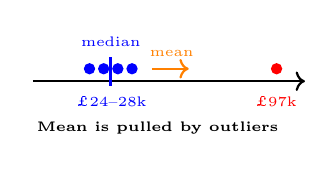
\begin{tikzpicture}[scale=0.72]
  \draw[thick,->] (-0.2,0) -- (4.6,0);
  \foreach \xd in {0.8, 1.05, 1.3, 1.55}{
    \fill[blue] (\xd,0.22) circle (0.1);
  }
  \fill[red] (4.1,0.22) circle (0.1);
  \node[below,font=\tiny,blue] at (1.2,{-0.1})  {£24--28k};
  \node[below,font=\tiny,red]  at (4.1,{-0.1})  {£97k};
  \draw[blue,very thick] (1.175,0.42) -- (1.175,-0.08);
  \node[above,blue,font=\tiny] at (1.175,0.44) {median};
  \draw[->,thick,orange] (1.9,0.22) -- (2.55,0.22);
  \node[above,orange,font=\tiny] at (2.25,0.26) {mean};
  \node[below,font=\tiny\bfseries] at (2.0,{-0.55})
    {Mean is pulled by outliers};
\end{tikzpicture}

\vspace{0.5em}


\end{center}

\column{0.67\textwidth}
\footnotesize
\vspace{0.3em}
\begin{enumerate}\itemsep1pt
  \begin{multicols}{2}
    \item $-6+(-2) = \ashowq{-8}$
    \item $\frac{1}{3}+\frac{1}{2} = \ashowq{\frac{5}{6}}$
  \end{multicols}
  \vspace{-1em}
  \item Median of: $3,\ 9,\ 4,\ 7,\ 1$ \ashow{4}
  \item Mean \textbf{and} median of: $5,\ 8,\ 3,\ 12,\ 7$. Which is larger? \ashow{equal (both $7$)}
  \item Five salaries are: £24k, £26k, £25k, £28k, \textcolor{red}{£97k}. Would you prefer to use the mean or the median to find the average? \ashow{the median}
  \item For $-10,-1,0,2,3$: \textit{estimate} whether the mean is positive or negative. Then calculate both mean and median. \ashow{negative: mean $-1.2$; median $0$}
  \item Find the mean and median of: $-6,\ -2,\ 4,\ -3,\ 7,\ 0$ \ashow{mean $0$; median $-1$}
  \item What is the median of: $\frac{1}{3},\ \frac{3}{4},\ \frac{1}{2},\ \frac{1}{6},\ \frac{2}{3},\ \frac{1}{4}$ \ashow{$\frac{5}{12}$}
  \item True or False?\\
    (a) The median is always one of the values in the dataset. \ashow{False}\\
    (b) The mean and median are always different. \ashow{False}\\
    (c) A very large outlier affects the median more than the mean. \ashow{False}

\end{enumerate}

\end{columns}
\end{frame}
\begin{frame}<1>{Starter}
\vspace{-0.8em}
\begin{columns}[T]

\column{0.33\textwidth}
\begin{center}

\vspace{7em}

% Dot plot showing mean pulled by outlier vs stable median
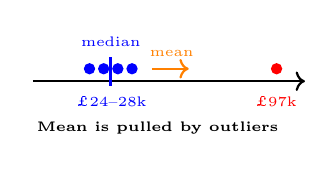
\begin{tikzpicture}[scale=0.72]
  \draw[thick,->] (-0.2,0) -- (4.6,0);
  \foreach \xd in {0.8, 1.05, 1.3, 1.55}{
    \fill[blue] (\xd,0.22) circle (0.1);
  }
  \fill[red] (4.1,0.22) circle (0.1);
  \node[below,font=\tiny,blue] at (1.2,{-0.1})  {£24--28k};
  \node[below,font=\tiny,red]  at (4.1,{-0.1})  {£97k};
  \draw[blue,very thick] (1.175,0.42) -- (1.175,-0.08);
  \node[above,blue,font=\tiny] at (1.175,0.44) {median};
  \draw[->,thick,orange] (1.9,0.22) -- (2.55,0.22);
  \node[above,orange,font=\tiny] at (2.25,0.26) {mean};
  \node[below,font=\tiny\bfseries] at (2.0,{-0.55})
    {Mean is pulled by outliers};
\end{tikzpicture}

\vspace{0.5em}


\end{center}

\column{0.67\textwidth}
\footnotesize
\vspace{0.3em}
\begin{enumerate}\itemsep1pt
  \begin{multicols}{2}
    \item $-6+(-2) = \ashowq{-8}$
    \item $\frac{1}{3}+\frac{1}{2} = \ashowq{\frac{5}{6}}$
  \end{multicols}
  \vspace{-1em}
  \item Median of: $3,\ 9,\ 4,\ 7,\ 1$ \ashow{4}
  \item Mean \textbf{and} median of: $5,\ 8,\ 3,\ 12,\ 7$. Which is larger? \ashow{equal (both $7$)}
  \item Five salaries are: £24k, £26k, £25k, £28k, \textcolor{red}{£97k}. Would you prefer to use the mean or the median to find the average? \ashow{the median}
  \item For $-10,-1,0,2,3$: \textit{estimate} whether the mean is positive or negative. Then calculate both mean and median. \ashow{negative: mean $-1.2$; median $0$}
  \item Find the mean and median of: $-6,\ -2,\ 4,\ -3,\ 7,\ 0$ \ashow{mean $0$; median $-1$}
  \item What is the median of: $\frac{1}{3},\ \frac{3}{4},\ \frac{1}{2},\ \frac{1}{6},\ \frac{2}{3},\ \frac{1}{4}$ \ashow{$\frac{5}{12}$}
  \item True or False?\\
    (a) The median is always one of the values in the dataset. \ashow{False}\\
    (b) The mean and median are always different. \ashow{False}\\
    (c) A very large outlier affects the median more than the mean. \ashow{False}

\end{enumerate}

\end{columns}
\end{frame}
\begin{frame}<1>{Starter}
\vspace{-0.8em}
\begin{columns}[T]

\column{0.33\textwidth}
\begin{center}

\vspace{7em}

% Dot plot showing mean pulled by outlier vs stable median
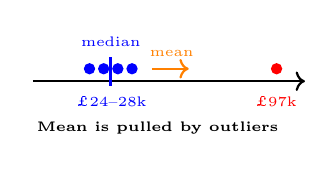
\begin{tikzpicture}[scale=0.72]
  \draw[thick,->] (-0.2,0) -- (4.6,0);
  \foreach \xd in {0.8, 1.05, 1.3, 1.55}{
    \fill[blue] (\xd,0.22) circle (0.1);
  }
  \fill[red] (4.1,0.22) circle (0.1);
  \node[below,font=\tiny,blue] at (1.2,{-0.1})  {£24--28k};
  \node[below,font=\tiny,red]  at (4.1,{-0.1})  {£97k};
  \draw[blue,very thick] (1.175,0.42) -- (1.175,-0.08);
  \node[above,blue,font=\tiny] at (1.175,0.44) {median};
  \draw[->,thick,orange] (1.9,0.22) -- (2.55,0.22);
  \node[above,orange,font=\tiny] at (2.25,0.26) {mean};
  \node[below,font=\tiny\bfseries] at (2.0,{-0.55})
    {Mean is pulled by outliers};
\end{tikzpicture}

\vspace{0.5em}


\end{center}

\column{0.67\textwidth}
\footnotesize
\vspace{0.3em}
\begin{enumerate}\itemsep1pt
  \begin{multicols}{2}
    \item $-6+(-2) = \ashowq{-8}$
    \item $\frac{1}{3}+\frac{1}{2} = \ashowq{\frac{5}{6}}$
  \end{multicols}
  \vspace{-1em}
  \item Median of: $3,\ 9,\ 4,\ 7,\ 1$ \ashow{4}
  \item Mean \textbf{and} median of: $5,\ 8,\ 3,\ 12,\ 7$. Which is larger? \ashow{equal (both $7$)}
  \item Five salaries are: £24k, £26k, £25k, £28k, \textcolor{red}{£97k}. Would you prefer to use the mean or the median to find the average? \ashow{the median}
  \item For $-10,-1,0,2,3$: \textit{estimate} whether the mean is positive or negative. Then calculate both mean and median. \ashow{negative: mean $-1.2$; median $0$}
  \item Find the mean and median of: $-6,\ -2,\ 4,\ -3,\ 7,\ 0$ \ashow{mean $0$; median $-1$}
  \item What is the median of: $\frac{1}{3},\ \frac{3}{4},\ \frac{1}{2},\ \frac{1}{6},\ \frac{2}{3},\ \frac{1}{4}$ \ashow{$\frac{5}{12}$}
  \item True or False?\\
    (a) The median is always one of the values in the dataset. \ashow{False}\\
    (b) The mean and median are always different. \ashow{False}\\
    (c) A very large outlier affects the median more than the mean. \ashow{False}

\end{enumerate}

\end{columns}
\end{frame}

\end{document}